\section{Lee's 3D Skeletonization}

\begin{frame}
  \frametitle{3D Skeletonization}
  \begin{block}
    {3D Skeleton}
    In 3D Euclidean space the skeleton of an object is the \textbf{locus of the centers} of all inscribed maximal spheres, where the spheres touch the boundary \textbf{at more than one point}.
  \end{block}
  A skeleton can be defined by \emph{medial axes} or \emph{medial surfaces}. We will focus on medial axes.
  \begin{columns}
    \begin{column}{0.5\textwidth}
      \begin{figure}
        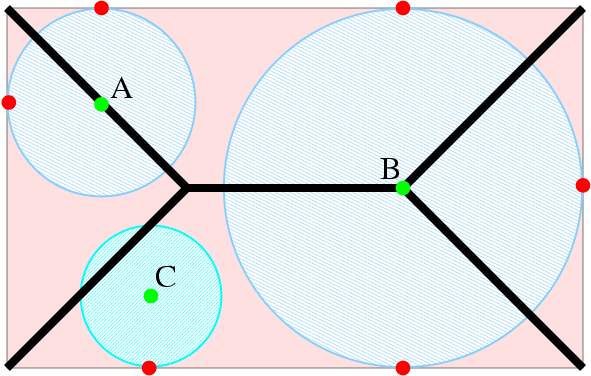
\includegraphics[width=0.7\textwidth]{skeltouch.png}
        \caption{2D representation of the above definition.}
      \end{figure}
    \end{column}
    \begin{column}{0.5\textwidth}
      \begin{figure}
        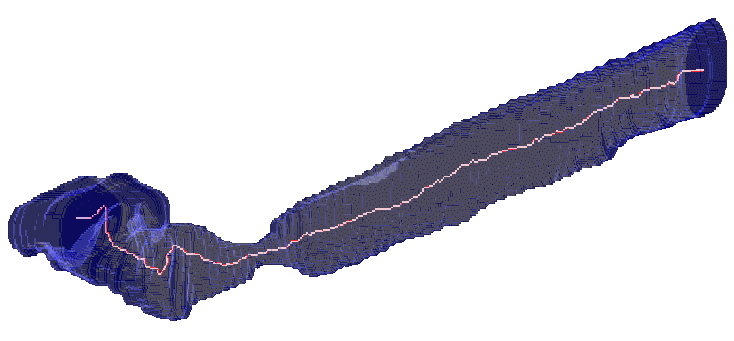
\includegraphics[width=0.9\textwidth]{tubular-skeleton.png}
        \caption{In white the medial axes skeleton of a 3D tubular object.}
      \end{figure}
    \end{column}
  \end{columns}
\end{frame}

\begin{frame}
  \frametitle{Topological properties}
  \begin{itemize}
    \item A 3D binary image is a 3D binary matrix of size $k_{max}\times j_{max} \times i_{max}$. Every pixel $v$ is represented by its coordinates $(k, j, i)$ and has the value $1$ or $0$.
    \item When we talk about 3D geometries we can describe them in terms of their topological properties such as the number of \emph{connected objects}, \emph{cavities} and \emph{holes}.
    \item The \textbf{Euler Characteristic} $\chi$ is a compact way combine those characteristics in a number that describes the geometry.
          \begin{equation}
            \chi(S) = O(S) - H(S) + C(S)
          \end{equation}
          where $O(S)$, $H(S)$ and $C(S)$ are the numbers of connected objects, holes and cavities of S, the set of all the points with the value 1.
    \item By using a local formula $G(S)$ for the Euler Characteristic, the complexity can be reduced by calculating $\chi(S)$ considering pixel by pixel neighbourhoods.
  \end{itemize}
\end{frame}
\begin{frame}
  \label{sli:euler-table}
  \frametitle{Neighborhoods}
  \begin{itemize}
    \item Considering a pixel $v$, its $26$-neighbours $N(v)$ are defined based on the cube below.
          \begin{columns}
            \begin{column}{0.5\textwidth}
              \begin{figure}
                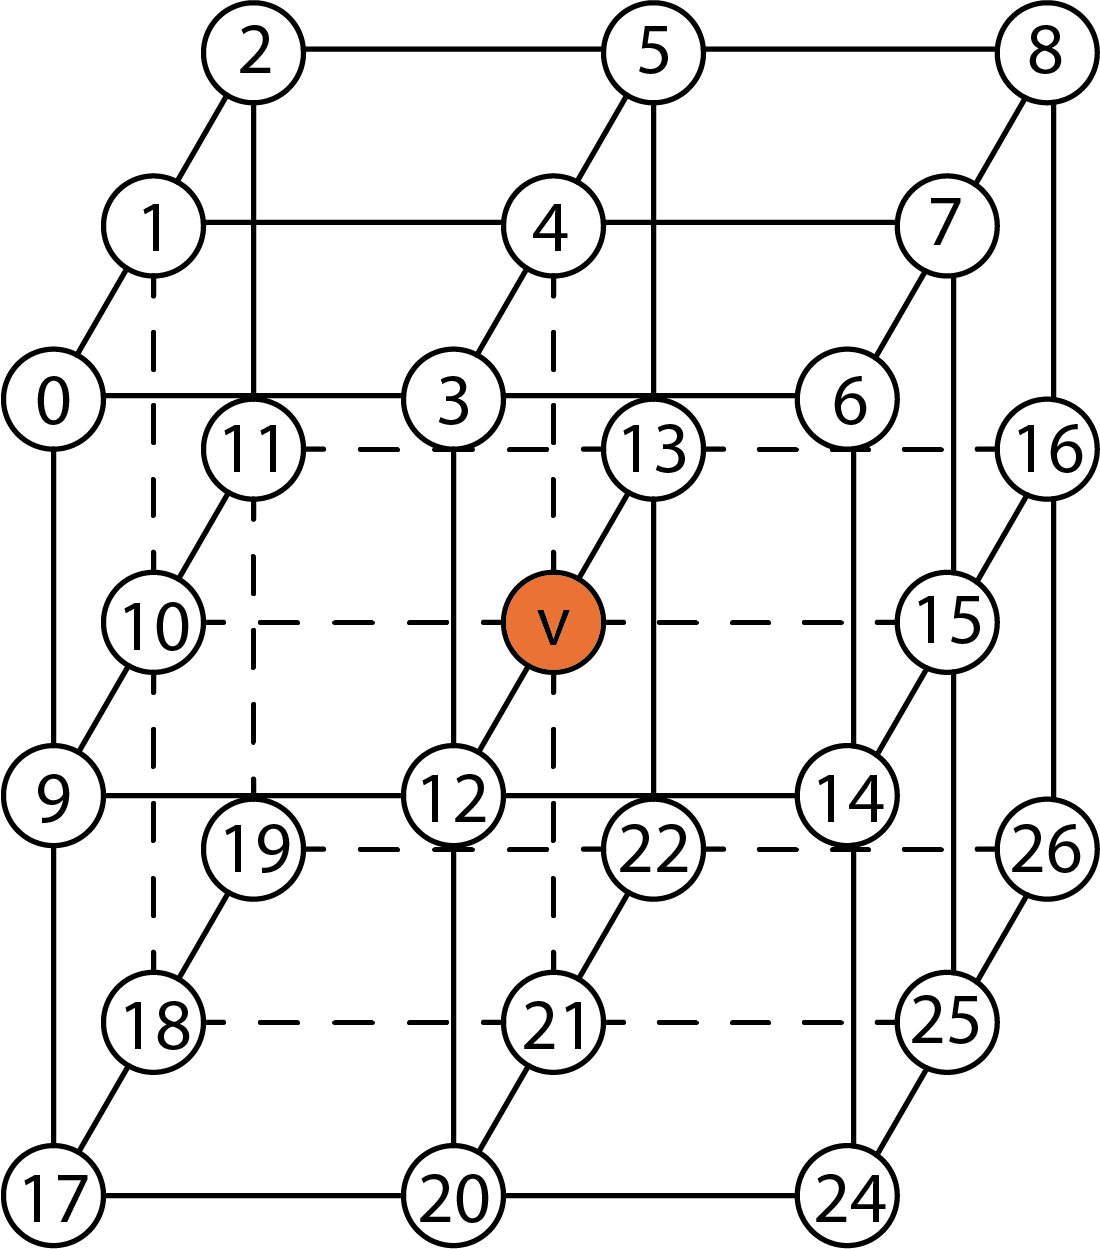
\includegraphics[width=0.5\textwidth]{neighbours-cube.png}
                \label{fig:cube-neighborhood}
              \end{figure}
              \begin{figure}
                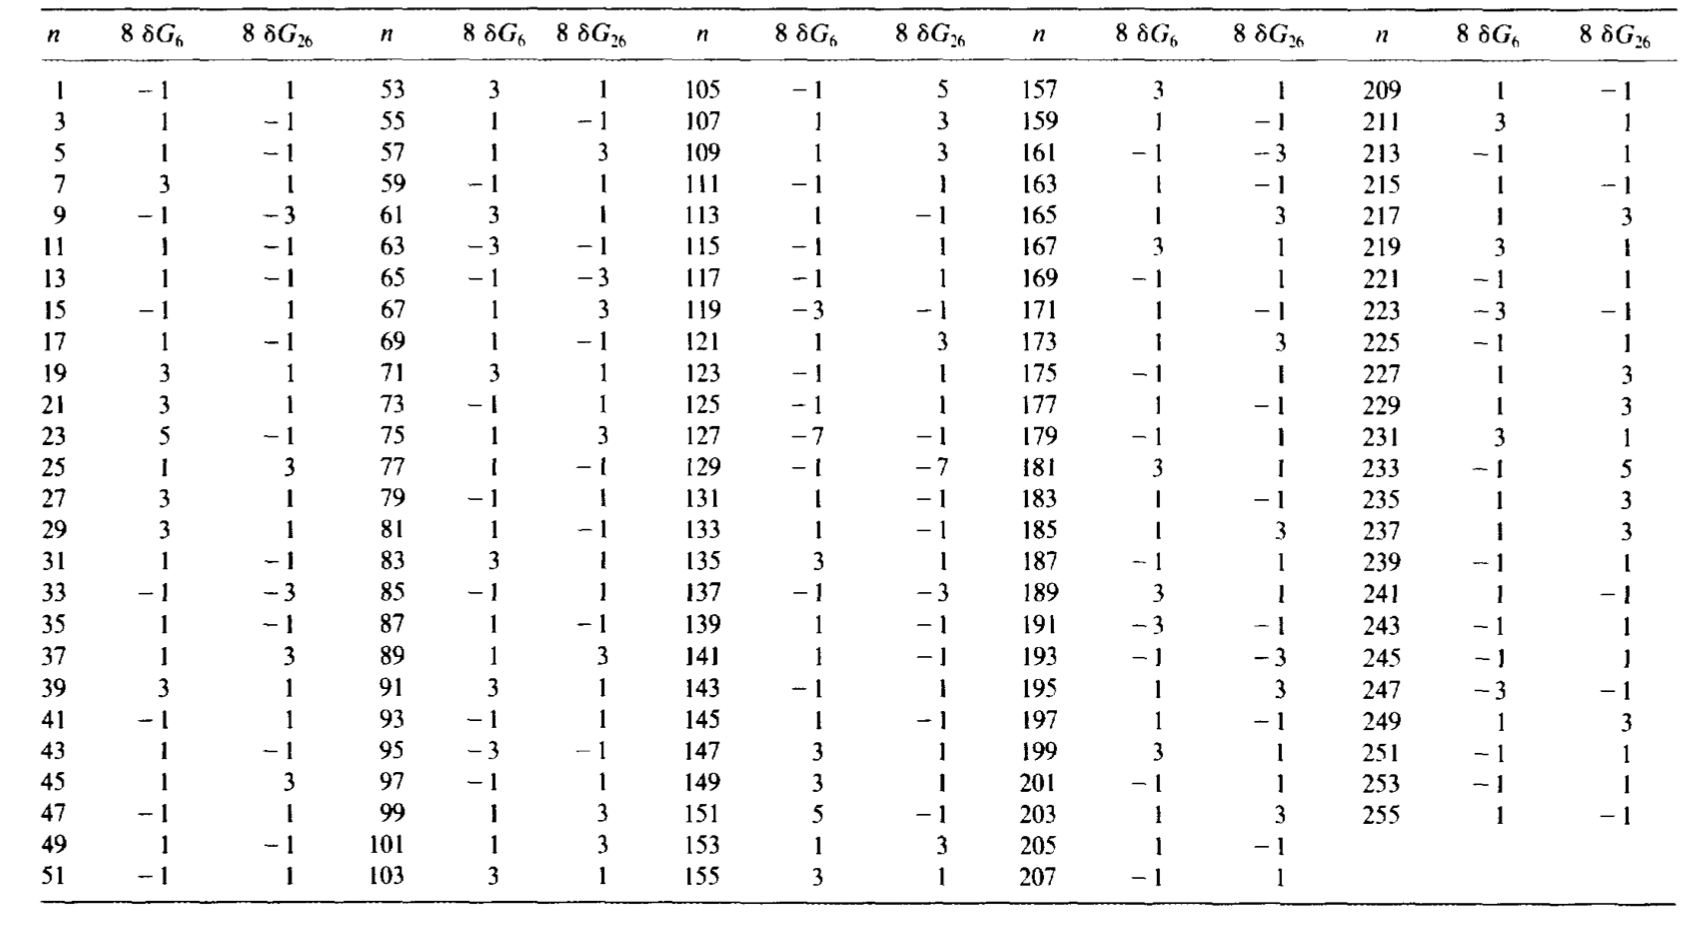
\includegraphics[width=\textwidth]{euler-invariance-table.png}
                \label{fig:euler-table}
              \end{figure}
            \end{column}
            \begin{column}{0.5\textwidth}
              \item This cube can be divided into eight overlapping $2\times2$ octants $N^2(v)$.
              \item Each octant have an Euler Characteristic value $G(N^2(v))$.
              \item Summing up each octant's $G(N^2(v))$ we obtain the \textbf{local Euler Characteristic} value for the pixel $v$.
              \item Since there are only 256 possible octant pixel configurations, we can store a \textbf{look-up table} to speed up computation.
            \end{column}
          \end{columns}
  \end{itemize}
\end{frame}

\begin{frame}
  \frametitle{Thinning}
  \begin{block}{Removing pixels}
    A pixel can be removed from the image (set to 0) if:
    \begin{itemize}
      \item is \textbf{not an endpoint} (endpoint if it has exactly one $1$-valued neighbour in the $26$-neighborhood).
      \item is \textbf{Euler-Invariant} (if removed the Euler Characteristic does not change).
      \item its removal \textbf{does not disconnect} the object.
    \end{itemize}
    A pixel with such characteristics is called \textbf{simple point}.
  \end{block}
  Simple point detection is a crucial step in Lee's 3D Skeletonization~\cite{lee94} algorithm.
  \begin{itemize}
    \item Euler-invariance can be checked efficiently using the Euler Table mentioned in Slide~\vref{sli:euler-table}.
    \item Connectivity can be determined using an \textbf{octree} data structure for representing the neighborhood $N(v)$.
  \end{itemize}
\end{frame}

\begin{frame}
  \frametitle{Connectivity checking}
  We can use a recursive procedure \lstinline{N(v)_labeling} to determine the number of connected objects in the $N(v)$ neighborhood if pixel $v$ is removed.
  \begin{figure}
    \centering
    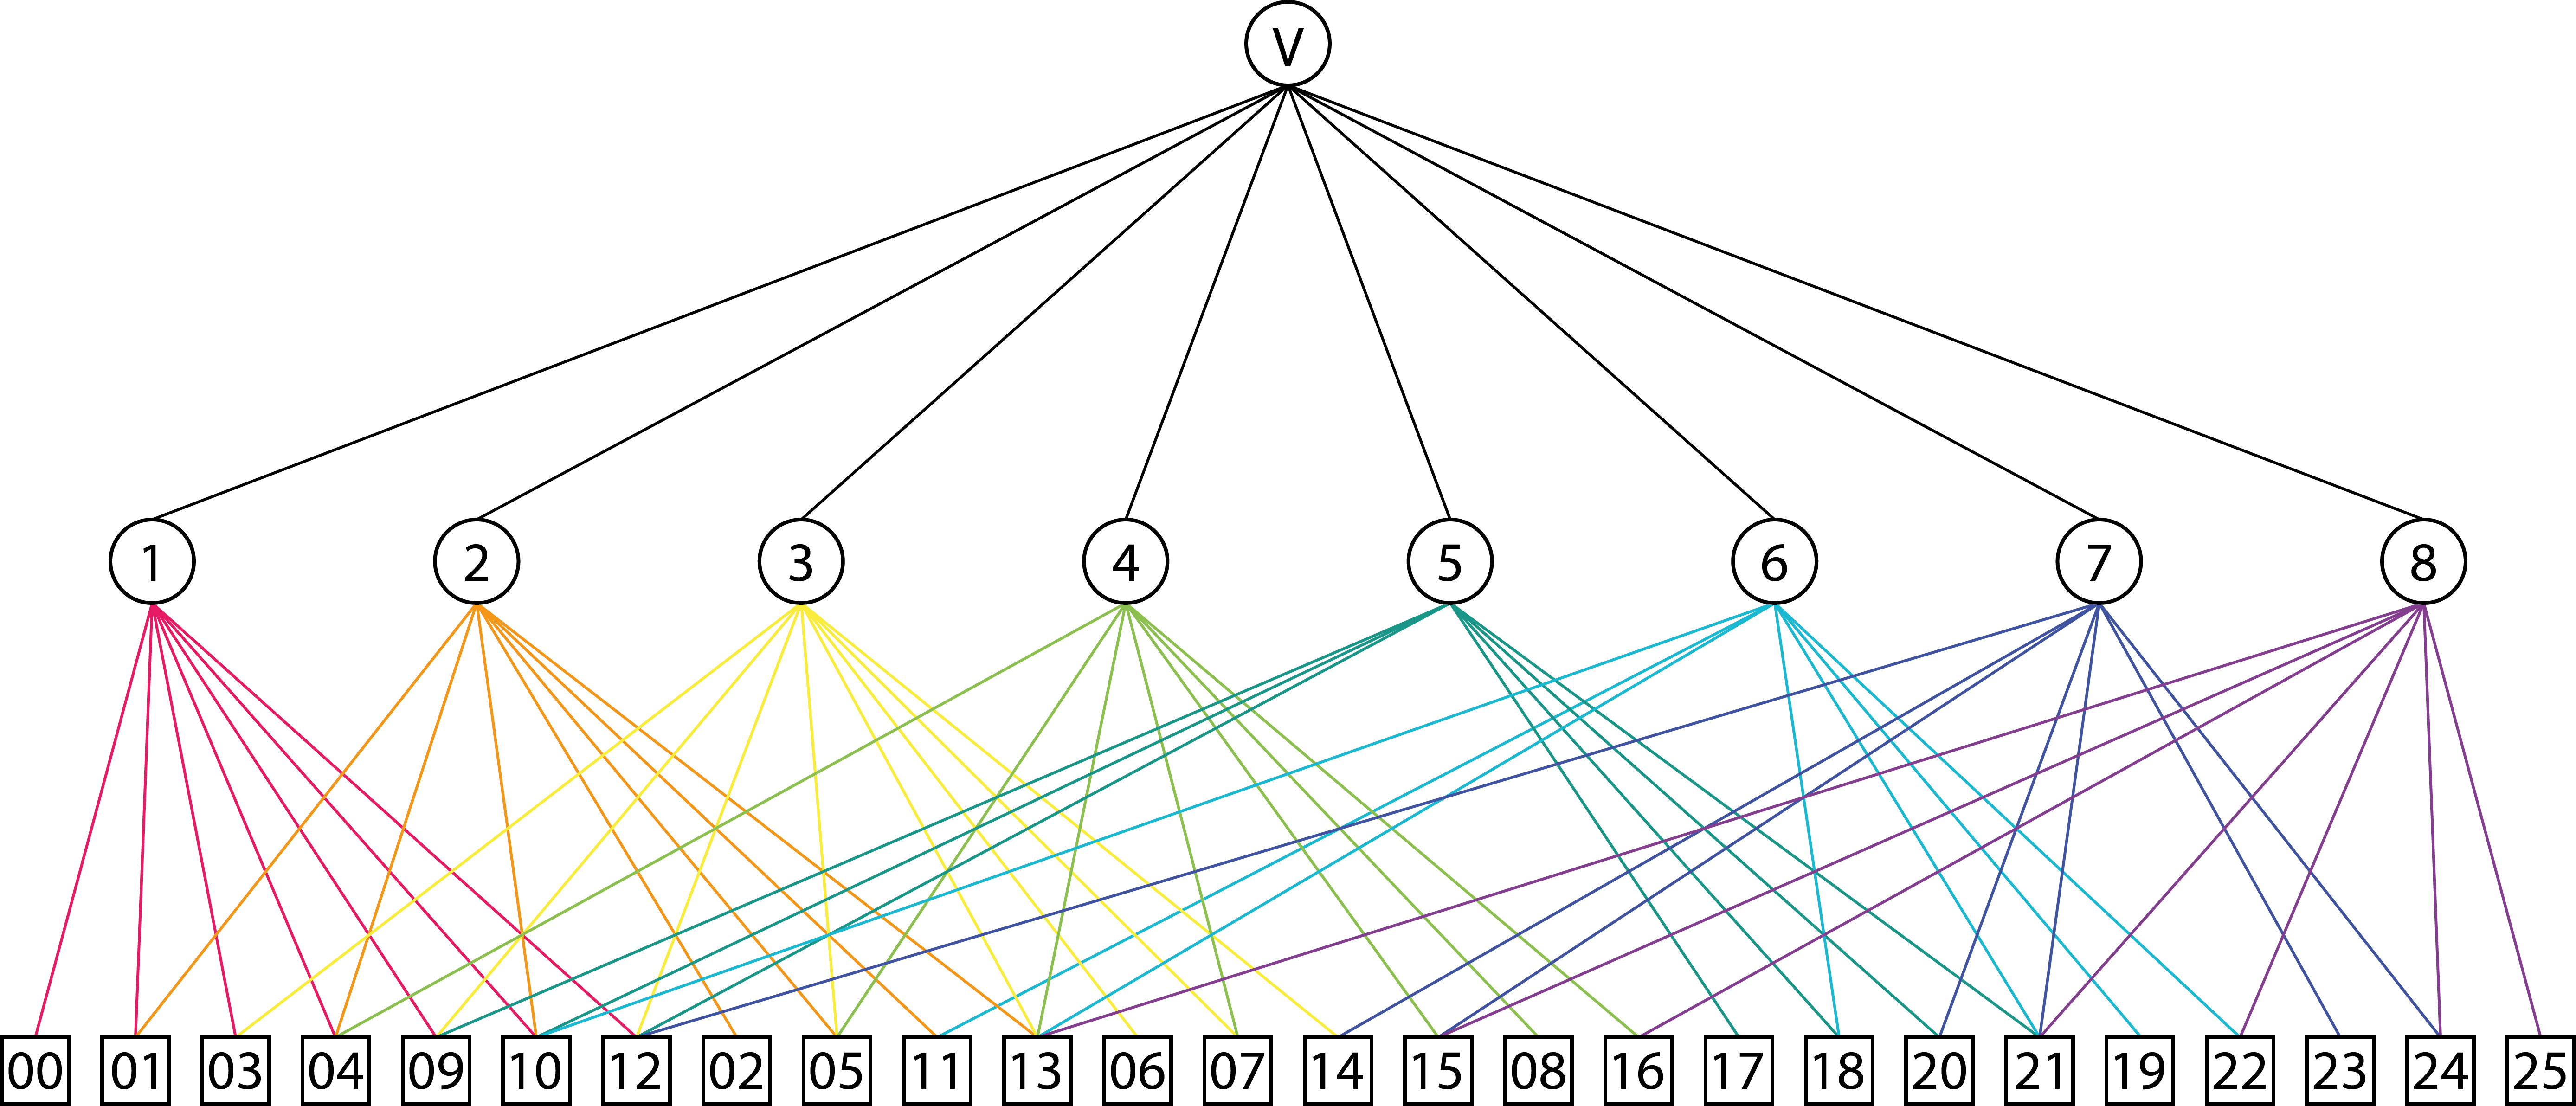
\includegraphics[width=0.7\textheight]{octree.png}
    \caption{Octree data structure for pixel $v$ and its 26-neighbohood.}
  \end{figure}
  \begin{itemize}
    \item The procedure recursively assigns labels to each pixel in the $26$-neighborhood.
    \item All connected pixels have the same label, i.e. each label represent a connected object.
    \item If more than one different label is assigned, there is more than one connected object.
  \end{itemize}
\end{frame}

\begin{frame}
  \frametitle{Lee's 3D Skeletonization Algorithm}
  \begin{block}{3D Skeletonization Algorithm}
    A thinning iteration is composed of the following phases:
    \begin{enumerate}
      \item For each one of the six directions (N, S, W, E, U, B):
            \begin{enumerate}
              \item Find a list of simple points candidates satisfying:
                    \begin{itemize}
                      \item Belongs to a border in the direction we're iterating on
                      \item Not an end point
                      \item Euler-Invariant
                      \item Preserve connectivity (through \lstinline{N(v)_labeling})
                    \end{itemize}
              \item For each simple point candidate:
                    \begin{enumerate}
                      \item Re-check if it preserve connectivity
                      \item if so delete it
                    \end{enumerate}
            \end{enumerate}
    \end{enumerate}
  \end{block}
  \begin{columns}
    \begin{column}[]{0.6\textwidth}
      \vspace{0.5cm}
      To apply Lee's algorithm on 2D images:
      \begin{itemize}
        \item add the third dimension by applying a padding of 0s.
        \item instead of iterating on the six directions, check only the four N, S, W, E.
      \end{itemize}
    \end{column}
    \begin{column}{0.4\textwidth}
      \begin{figure}
        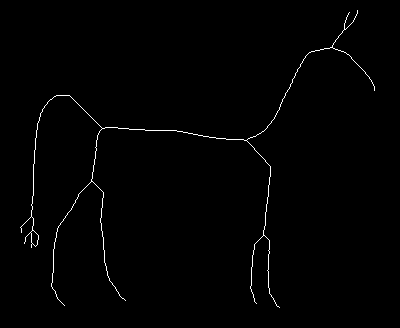
\includegraphics[width=0.65\textwidth]{lee-skeleton.png}
        \caption{Lee's skeleton of our horse.}
      \end{figure}
    \end{column}
  \end{columns}

\end{frame}
